\documentclass{article}\usepackage[]{graphicx}\usepackage[]{color}
% maxwidth is the original width if it is less than linewidth
% otherwise use linewidth (to make sure the graphics do not exceed the margin)
\makeatletter
\def\maxwidth{ %
  \ifdim\Gin@nat@width>\linewidth
    \linewidth
  \else
    \Gin@nat@width
  \fi
}
\makeatother

\definecolor{fgcolor}{rgb}{0.345, 0.345, 0.345}
\newcommand{\hlnum}[1]{\textcolor[rgb]{0.686,0.059,0.569}{#1}}%
\newcommand{\hlstr}[1]{\textcolor[rgb]{0.192,0.494,0.8}{#1}}%
\newcommand{\hlcom}[1]{\textcolor[rgb]{0.678,0.584,0.686}{\textit{#1}}}%
\newcommand{\hlopt}[1]{\textcolor[rgb]{0,0,0}{#1}}%
\newcommand{\hlstd}[1]{\textcolor[rgb]{0.345,0.345,0.345}{#1}}%
\newcommand{\hlkwa}[1]{\textcolor[rgb]{0.161,0.373,0.58}{\textbf{#1}}}%
\newcommand{\hlkwb}[1]{\textcolor[rgb]{0.69,0.353,0.396}{#1}}%
\newcommand{\hlkwc}[1]{\textcolor[rgb]{0.333,0.667,0.333}{#1}}%
\newcommand{\hlkwd}[1]{\textcolor[rgb]{0.737,0.353,0.396}{\textbf{#1}}}%
\let\hlipl\hlkwb

\usepackage{framed}
\makeatletter
\newenvironment{kframe}{%
 \def\at@end@of@kframe{}%
 \ifinner\ifhmode%
  \def\at@end@of@kframe{\end{minipage}}%
  \begin{minipage}{\columnwidth}%
 \fi\fi%
 \def\FrameCommand##1{\hskip\@totalleftmargin \hskip-\fboxsep
 \colorbox{shadecolor}{##1}\hskip-\fboxsep
     % There is no \\@totalrightmargin, so:
     \hskip-\linewidth \hskip-\@totalleftmargin \hskip\columnwidth}%
 \MakeFramed {\advance\hsize-\width
   \@totalleftmargin\z@ \linewidth\hsize
   \@setminipage}}%
 {\par\unskip\endMakeFramed%
 \at@end@of@kframe}
\makeatother

\definecolor{shadecolor}{rgb}{.97, .97, .97}
\definecolor{messagecolor}{rgb}{0, 0, 0}
\definecolor{warningcolor}{rgb}{1, 0, 1}
\definecolor{errorcolor}{rgb}{1, 0, 0}
\newenvironment{knitrout}{}{} % an empty environment to be redefined in TeX

\usepackage{alltt}
\usepackage{Sweave}
\usepackage{float}
\usepackage{subcaption}
\usepackage{graphicx}
\usepackage{tabularx}
\usepackage{siunitx}
\usepackage{multirow}
\usepackage{amssymb} % for math symbols
\usepackage{amsmath} % for aligning equations
%\usepackage{hyperref}
\usepackage{textcomp}
\usepackage{mdframed}
\usepackage{longtable}
\usepackage{natbib}
\bibliographystyle{..//bib/styles/gcb}
%\usepackage[hyphens]{url}
\usepackage{caption}
\setlength{\captionmargin}{30pt}
\setlength{\abovecaptionskip}{0pt}
\setlength{\belowcaptionskip}{10pt}
\topmargin -1.5cm        
\oddsidemargin -0.04cm   
\evensidemargin -0.04cm
\textwidth 16.59cm
\textheight 21.94cm 
%\pagestyle{empty} %comment if want page numbers
\parskip 7.2pt
\renewcommand{\baselinestretch}{1}
\parindent 0pt
\usepackage{lineno}
\linenumbers

%cross referencing:
\usepackage{xr}
\externaldocument{regrisk}

\newmdenv[
  topline=true,
  bottomline=true,
  skipabove=\topsep,
  skipbelow=\topsep
]{siderules}

%% R Script


\IfFileExists{upquote.sty}{\usepackage{upquote}}{}
\begin{document}
\noindent 
\textbf{\LARGE{Supplemental Materials: Climate change reshapes the drivers of false spring risk across European trees}} 
%\\
%OR \\
%\textbf{\Large{Climate change increases the risk of false springs in European trees}} \\ % Lizzie votes for the first title! Reviewers can ask you to make it more narrow so I would start here and shift to Ben's if requested ... (goal 1: get paper out for review)
%\textbf{\Large{False spring risk increases across European trees in the face of climate change}}



\noindent Authors:\\
C. J. Chamberlain $^{1,2}$, B. I. Cook $^{3}$, I. Morales-Castilla $^{4,5}$ \& E. M. Wolkovich $^{1,2,6}$
\vspace{2ex}\\
\emph{Author affiliations:}\\
$^{1}$Arnold Arboretum of Harvard University, 1300 Centre Street, Boston, Massachusetts, USA; \\
$^{2}$Organismic \& Evolutionary Biology, Harvard University, 26 Oxford Street, Cambridge, Massachusetts, USA; \\
$^{3}$NASA Goddard Institute for Space Studies, New York, New York, USA; \\
$^{4}$GloCEE - Global Change Ecology and Evolution Group, Department of Life Sciences, Universidad de Alcal\'{a}, Alcal\'{a} de Henares, 28805, Spain \\
$^{5}$Department of Environmental Science and Policy, George Mason University, Fairfax, VA 22030; \\
$^{6}$Forest \& Conservation Sciences, Faculty of Forestry, University of British Columbia, 2424 Main Mall, Vancouver, BC V6T 1Z4\\
\vspace{2ex}
$^*$Corresponding author: 248.953.0189; cchamberlain@g.harvard.edu\\

\renewcommand{\thetable}{S\arabic{table}}
\renewcommand{\thefigure}{S\arabic{figure}}
\renewcommand{\labelitemi}{$-$}
\setkeys{Gin}{width=0.8\textwidth}

\section*{Methods: Space predictor} %I'm not too sure about the 'space parameter' terminology, I'd rather use either spatial or geographic predictor or proxy. I'm using spatial predictor, but all our predictors are spatial, so please feel free to change.

Spatial autocorrelation (SA) is a common issue in spatial ecology given that nearby spatial units tend to be more similar than units far apart, and thus, cannot be considered as independent units, which is a frequent assumption in statistical tests \citep{diniz2003spatial}. If model residuals are spatially autocorrelated, and thus, non-independent then model coefficients and errors may be biased in a hard-to-predict way \citep{mauricio2009coefficient}. On the contrary, if model residuals are not autocorrelated, then SA should not be of concern \citep{hawkins2012eight}.\\

To control for spatial autocorrelation and to account for spatially structured processes independent from our environmental predictors of false springs, we generated an additional spatial predictor for the model. To avoid collinearity, we computed our spatial predictor from the residuals of a linear model of false springs as a function (Equation S1) of all other factors that are also spatially structured (e.g. spring temperature, altitude, distance to the coast), following the logic of spatial filter modelling \citep{diniz2005modelling}. The calculation of the spatial predictor followed the next steps: (a) we fit a linear model of false spring versus environmental factors, (b) we extracted the residuals of the regression Equation S1, which represent the portion of the variation in the number of false springs that is independent from the predictors in the model and (c) we utilized the residuals as our \textit{y\textsubscript{i}} values in a selection of spatial eigenvectors to retain only the minimal subset of spatial eigenvectors that are able to remove SA from model residuals. Specifically, we selected eigenvectors following the the minimization of Moran's \textit{I} of the residuals (MIR) approach \citep{griffith2006spatial,diniz2012selection,Baumen2017}. (d) Next, we fit a linear model between the residuals of Equation S1 and the subset of selected eigenvectors. And, finally, (e) we took the fitted values from this regression as our spatial predictor in our final model (see equation from main text, Equation 1), which can be interpreted as a latent variable summarizing the spatial structure in false springs that is unaccounted for by the rest of the environmental factors in our model \citep{morales2012imprint}. 

\begin{align*}
y_i = \alpha_{[i]} +&  \beta_{NAO_{[i]}} + \beta_{MST_{[i]}} + \beta_{Elevation_{[i]}} + \beta_{DistanceCoast_{[i]}} \\ +& \beta_{ClimateChange_{[i]}}
+ \beta_{NAO \times Species_{[i]}} + \beta_{MST \times Species_{[i]}} + \beta_{Elevation \times Species_{[i]}} \\ +& \beta_{DistanceCoast \times Species_{[i]}} + \beta_{ClimateChange \times Species_{[i]}} \\
+& \beta_{NAO \times ClimateChange_{[i]}} + \beta_{MST \times ClimateChange_{[i]}} 
+ \beta_{Elevation \times ClimateChange_{[i]}} \\ +& \beta_{DistanceCoast \times ClimateChange_{[i]}} + \sigma_{[i]} \tag{S1}
\end{align*}


\section*{Species rate of budburst calculations}
Due to the paucity of data for BBCH 7 in the PEP725 dataset, we were unable to use observations for both budburst and leafout to determine the durations of vegetative risk. Instead, we used data from a growth chamber experiment \citep{Flynn2018} to determine the average number of days between budburst and leafout for our study species. We took the mean number of days between budburst and leafout for the entire experiment, which was 12 days. We compared this number to a field observation study \citep{Donnelly2017} that looked at the time between budburst and leafout across 10 species over 5 years. Finally, we assessed data that were provided by the USA National Phenology Network and the many participants who contribute to its Nature's Notebook program (USA-NPN,2019; www.usanpn.org/data/observational) for \textit{Aesculus flava} (Sol.), \textit{Aesculus glabra} (Willd.), \textit{Alnus incana} (Moench.), \textit{Betula nigra} (L.), \textit{Betula papyrifera} (Marshall), \textit{Fagus grandifolia} (Ehrh.), \textit{Fraxinus americana} (L.), \textit{Fraxinus nigra} (Marshall) and \textit{Quercus velutina} (Lam.) and took the mean number of days between budburst and leafout. Across all three approaches, the average number of days between budburst and leafout was approximately 12 days. Thus, we expanded our rate of budburst through full leaf expansion by subtracting 12 days from the first leaf to find budburst and adding 12 days to the first leaf to find full leafout. 

Again, due to a lack of BBCH 7 data, we were unable to determine species-specific averages of number of days between budburst and leafout. We used a similar approach as above by using data from the growth chamber experiment \citep{Flynn2018} but instead of finding whole experiment means we determined species-specific averages. We used the rate of budburst of \textit{Acer saccharum} (Marshall) for \textit{Aesculus hippocastanum} \citep{Buerki2010}, \textit{Alnus incana} for \textit{Alnus glutinosa}, \textit{Betula papyrifera} for \textit{Betula pendula} \citep{Wang2016}, \textit{Fagus grandifolia} for \textit{Fagus sylvatica}, \textit{Fraxinus nigra} for \textit{Fraxinus excelsior} and \textit{Quercus alba} (L.) for \textit{Quercus robur} \citep{Hipp2017}.

%NOT SURE WHERE TO PUT THIS!!
%Most species had mean spring temperatures that ranged from -5$^{\circ}$C to 12$^{\circ}$C, but for \textit{Alnus glutinosa} and \textit{Fraxinus excelsior} temperatures rarely dropped below 0$^{\circ}$C, whereas \textit{Quercus robur} experienced some of the lowest spring temperatures (see Figure S1). 

\iffalse
\begin{align*}
inverselogit = & (1/(1+exp(-(Model Estimate)))) \tag{S2} 
\end{align*}
\begin{align*}
inverselogit(Intercept &+ (Model Estimate/(sd(Raw Data Predictor)*2))*mean(Raw Data Predictor)) - \\ & inverselogit(Intercept + (Model Estimate/(sd(Raw Data Predictor)*2)) \\ & *(mean(Raw Data Predictor)-(2*sd(Raw Data Predictor))) * 100 \tag{S3} 
\end{align*}
\fi

\newpage
\nocite{NPN2019}
\bibliography{..//bib/regionalrisk.bib}

\newpage
\section*{Supplement: Tables and Figures}
  
\begin{center}
\captionof{table}{Data collected from PEP725 for each species and the calculated number of false spring years} \label{tab:spp} 
\begin{tabular}{l r r r r}
\hline
Species & Num. of Observations & Num. of False Springs & Num. of Sites & Num. of Years \\
\hline
\textit{Aesculus hippocastanum} & 156468 & 44746 & 10157 & 66  \\
\textit{Alnus glutinosa} & 91094 & 27296 & 6775 & 65 \\
\textit{Betula pendula} & 154897 & 46685 & 10139 & 66 \\
\textit{Fagus sylvatica} & 129133 & 29237 & 9099 & 66 \\
\textit{Fraxinus excelsior} & 92665 & 8256 & 7327 & 65 \\
\textit{Quercus robur} & 131635 & 16657 & 8811 & 66 \\
\hline
\end{tabular}
\end{center}

\vspace{15ex}




\begin{center}
\captionof{table}{Mean day of budburst and standard deviation for each species for before (1951-1983) and after recent climate change (1984-2016).} \label{tab:bbspp}
\begin{tabular}{l c c| c c}
\cline{2-5}
& \multicolumn{2}{ c| }{1951-1983}
& \multicolumn{2}{ c }{1984-2016} \\ \cline{2-5}
& mean & sd & mean & sd \\
\hline
\textit{Aesculus hippocastanum} & 102.2 & 12.44 & 95.35 & 12.09  \\
\textit{Alnus glutinosa} & 102.8 & 14.81 & 94.90 & 14.71 \\
\textit{Betula pendula} & 101.3 & 11.76 & 95.44 & 11.25 \\
\textit{Fagus sylvatica} & 109.1 & 9.978 & 103.7 & 9.623 \\
\textit{Fraxinus excelsior} & 119.4 & 11.79 & 113.5 & 11.53 \\
\textit{Quercus robur} & 115.9 & 11.31 & 109.6 & 10.95 \\
\hline
\end{tabular}
\end{center}


% latex table generated in R 3.6.0 by xtable 1.8-4 package
% Fri May 29 07:57:10 2020
\begin{table}[H]
\centering
\caption{Summary of simple linear regression model of day of budburst before and after climate change across species.} 
\label{tab:simbbmod}
\begin{tabular}{lrrr}
  \hline
 & mean & 2\% & 98\% \\ 
  \hline
Intercept & 102.27 & 102.18 & 102.36 \\ 
  Climate Change & -6.98 & -7.13 & -6.84 \\ 
  \textit{Alnus glutinosa} & 0.61 & 0.45 & 0.77 \\ 
  \textit{Betula pendula} & -0.89 & -1.02 & -0.76 \\ 
  \textit{Fagus sylvatica} & 6.85 & 6.71 & 6.98 \\ 
  \textit{Fraxinus excelsior} & 17.16 & 17.01 & 17.33 \\ 
  \textit{Quercus robur} & 13.67 & 13.53 & 13.81 \\ 
  Climate Change x \textit{Alnus glutinosa} & -0.97 & -1.20 & -0.74 \\ 
  Climate Change x \textit{Betula pendula} & 1.06 & 0.86 & 1.26 \\ 
  Climate Change x \textit{Fagus sylvatica} & 1.61 & 1.41 & 1.82 \\ 
  Climate Change x \textit{Fraxinus excelsior} & 1.07 & 0.84 & 1.30 \\ 
  Climate Change x \textit{Quercus robur} & 0.67 & 0.46 & 0.88 \\ 
   \hline
\end{tabular}
\end{table}


% latex table generated in R 3.6.0 by xtable 1.8-4 package
% Fri May 29 07:57:11 2020
\begin{table}[H]
\centering
\caption{Summary of simple linear regression model of average minimum temperature between budburst and leafout before and after climate change across species.} 
\label{tab:simptmin}
\begin{tabular}{lrrr}
  \hline
 & mean & 2\% & 98\% \\ 
  \hline
Intercept & 5.99 & 5.97 & 6.00 \\ 
  Climate Change & 0.83 & 0.80 & 0.85 \\ 
  \textit{Alnus glutinosa} & 1.65 & 1.62 & 1.68 \\ 
  \textit{Betula pendula} & 0.50 & 0.48 & 0.53 \\ 
  \textit{Fagus sylvatica} & 1.50 & 1.47 & 1.52 \\ 
  \textit{Fraxinus excelsior} & 2.76 & 2.73 & 2.79 \\ 
  \textit{Quercus robur} & 1.88 & 1.86 & 1.91 \\ 
  Climate Change x \textit{Alnus glutinosa} & -0.04 & -0.08 & 0.01 \\ 
  Climate Change x \textit{Betula pendula} & -0.31 & -0.35 & -0.27 \\ 
  Climate Change x \textit{Fagus sylvatica} & 0.08 & 0.04 & 0.11 \\ 
  Climate Change x \textit{Fraxinus excelsior} & -0.26 & -0.30 & -0.22 \\ 
  Climate Change x \textit{Quercus robur} & -0.10 & -0.14 & -0.06 \\ 
   \hline
\end{tabular}
\end{table}


% latex table generated in R 3.6.0 by xtable 1.8-4 package
% Fri May 29 07:57:12 2020
\begin{table}[H]
\centering
\caption{Summary of simple linear regression model of the number of false springs before and after climate change across species.} 
\label{tab:simpfs}
\begin{tabular}{lrrr}
  \hline
 & mean & 2\% & 98\% \\ 
  \hline
Intercept & 5.56 & 5.52 & 5.59 \\ 
  Climate Change & 1.26 & 1.21 & 1.30 \\ 
  \textit{Alnus glutinosa} & -1.22 & -1.27 & -1.17 \\ 
  \textit{Betula pendula} & 0.13 & 0.09 & 0.17 \\ 
  \textit{Fagus sylvatica} & -0.94 & -0.98 & -0.89 \\ 
  \textit{Fraxinus excelsior} & -3.73 & -3.78 & -3.68 \\ 
  \textit{Quercus robur} & -2.98 & -3.03 & -2.94 \\ 
  Climate Change x \textit{Alnus glutinosa} & 1.21 & 1.14 & 1.28 \\ 
  Climate Change x \textit{Betula pendula} & 0.08 & 0.01 & 0.15 \\ 
  Climate Change x \textit{Fagus sylvatica} & -1.41 & -1.48 & -1.34 \\ 
  Climate Change x \textit{Fraxinus excelsior} & -1.56 & -1.64 & -1.49 \\ 
  Climate Change x \textit{Quercus robur} & -1.43 & -1.50 & -1.36 \\ 
   \hline
\end{tabular}
\end{table}


\newpage
% latex table generated in R 3.6.0 by xtable 1.8-4 package
% Fri May 29 07:57:12 2020
\begin{longtable}{lrrrrrrr}
\caption{Summary of Bernoulli model with the effects of species, climatic and geographical predictors on false spring risk.} \\ 
  \hline
 & mean & 2\% & 10\% & 25\% & 75\% & 90\% & 98\% \\ 
  \hline \endhead  \hline
Intercept & -0.42 & -0.43 & -0.43 & -0.42 & -0.41 & -0.41 & -0.41 \\ 
  NAO Index & 0.26 & 0.23 & 0.24 & 0.25 & 0.26 & 0.28 & 0.28 \\ 
  Mean Spring 
Temperature & -0.20 & -0.24 & -0.23 & -0.21 & -0.19 & -0.18 & -0.17 \\ 
  Distance from 
Coast & 0.28 & 0.25 & 0.26 & 0.27 & 0.29 & 0.31 & 0.32 \\ 
  Elevation & 0.29 & 0.25 & 0.26 & 0.28 & 0.30 & 0.32 & 0.33 \\ 
  Space Parameter & -0.01 & -0.04 & -0.03 & -0.02 & -0.01 & 0.00 & 0.01 \\ 
  Climate Change & 0.12 & 0.09 & 0.10 & 0.11 & 0.13 & 0.14 & 0.15 \\ 
  \textit{Alnus glutinosa} & 0.02 & -0.00 & 0.01 & 0.01 & 0.03 & 0.03 & 0.04 \\ 
  \textit{Betula pendula} & 0.08 & 0.06 & 0.07 & 0.07 & 0.08 & 0.09 & 0.10 \\ 
  \textit{Fagus sylvatica} & -0.54 & -0.56 & -0.56 & -0.55 & -0.54 & -0.53 & -0.52 \\ 
  \textit{Fraxinus excelsior} & -1.68 & -1.71 & -1.70 & -1.69 & -1.67 & -1.66 & -1.65 \\ 
  \textit{Quercus robur} & -1.26 & -1.28 & -1.27 & -1.26 & -1.25 & -1.24 & -1.23 \\ 
  NAO Index
x\textit{ Alnus glutinosa} & -0.10 & -0.15 & -0.13 & -0.11 & -0.09 & -0.07 & -0.05 \\ 
  NAO Index
x\textit{ Betula pendula} & -0.07 & -0.11 & -0.09 & -0.08 & -0.06 & -0.04 & -0.03 \\ 
  NAO Index
x\textit{ Fagus sylvatica} & 0.08 & 0.03 & 0.05 & 0.07 & 0.09 & 0.11 & 0.12 \\ 
  NAO Index
x\textit{ Fraxinus excelsior} & -0.08 & -0.15 & -0.13 & -0.10 & -0.06 & -0.04 & -0.02 \\ 
  NAO Index
x\textit{ Quercus robur} & -0.01 & -0.06 & -0.04 & -0.02 & 0.01 & 0.03 & 0.05 \\ 
  Mean Spring 
Temperature
x\textit{ Alnus glutinosa} & 0.18 & 0.13 & 0.14 & 0.16 & 0.20 & 0.22 & 0.23 \\ 
  Mean Spring 
Temperature
x\textit{ Betula pendula} & -0.02 & -0.06 & -0.05 & -0.03 & -0.00 & 0.01 & 0.03 \\ 
  Mean Spring 
Temperature
x\textit{ Fagus sylvatica} & -0.16 & -0.21 & -0.20 & -0.18 & -0.15 & -0.13 & -0.12 \\ 
  Mean Spring 
Temperature
x\textit{ Fraxinus excelsior} & 0.26 & 0.18 & 0.21 & 0.24 & 0.28 & 0.31 & 0.34 \\ 
  Mean Spring 
Temperature
x\textit{ Quercus robur} & 0.04 & -0.01 & 0.00 & 0.03 & 0.06 & 0.08 & 0.10 \\ 
  Distance from 
Coast
x\textit{ Alnus glutinosa} & -0.04 & -0.10 & -0.08 & -0.06 & -0.03 & -0.00 & 0.01 \\ 
  Distance from 
Coast
x\textit{ Betula pendula} & 0.01 & -0.03 & -0.02 & 0.00 & 0.03 & 0.05 & 0.06 \\ 
  Distance from 
Coast
x\textit{ Fagus sylvatica} & 0.11 & 0.06 & 0.07 & 0.09 & 0.12 & 0.15 & 0.16 \\ 
  Distance from 
Coast
x\textit{ Fraxinus excelsior} & 0.34 & 0.27 & 0.29 & 0.32 & 0.37 & 0.40 & 0.42 \\ 
  Distance from 
Coast
x\textit{ Quercus robur} & 0.00 & -0.06 & -0.04 & -0.01 & 0.02 & 0.05 & 0.06 \\ 
  Elevation
x\textit{ Alnus glutinosa} & 0.06 & -0.00 & 0.02 & 0.04 & 0.08 & 0.11 & 0.13 \\ 
  Elevation
x\textit{ Betula pendula} & 0.05 & -0.00 & 0.01 & 0.03 & 0.06 & 0.08 & 0.10 \\ 
  Elevation
x\textit{ Fagus sylvatica} & -0.03 & -0.09 & -0.07 & -0.05 & -0.01 & 0.01 & 0.02 \\ 
  Elevation
x\textit{ Fraxinus excelsior} & -0.34 & -0.43 & -0.40 & -0.37 & -0.32 & -0.28 & -0.26 \\ 
  Elevation
x\textit{ Quercus robur} & -0.10 & -0.16 & -0.15 & -0.12 & -0.08 & -0.06 & -0.04 \\ 
  Space Parameter
x\textit{ Alnus glutinosa} & 0.01 & -0.03 & -0.02 & 0.00 & 0.02 & 0.04 & 0.05 \\ 
  Space Parameter
x\textit{ Betula pendula} & -0.01 & -0.05 & -0.04 & -0.02 & -0.00 & 0.01 & 0.02 \\ 
  Space Parameter
x\textit{ Fagus sylvatica} & -0.05 & -0.09 & -0.08 & -0.07 & -0.04 & -0.03 & -0.02 \\ 
  Space Parameter
x\textit{ Fraxinus excelsior} & 0.03 & -0.03 & -0.01 & 0.01 & 0.05 & 0.07 & 0.09 \\ 
  Space Parameter
x\textit{ Quercus robur} & 0.00 & -0.04 & -0.03 & -0.01 & 0.01 & 0.03 & 0.05 \\ 
  Climate Change
x\textit{ Alnus glutinosa} & 0.06 & 0.01 & 0.02 & 0.04 & 0.07 & 0.09 & 0.10 \\ 
  Climate Change
x\textit{ Betula pendula} & 0.04 & 0.00 & 0.02 & 0.03 & 0.05 & 0.07 & 0.08 \\ 
  Climate Change
x\textit{ Fagus sylvatica} & -0.30 & -0.34 & -0.33 & -0.31 & -0.28 & -0.27 & -0.25 \\ 
  Climate Change
x\textit{ Fraxinus excelsior} & -0.40 & -0.46 & -0.44 & -0.41 & -0.38 & -0.35 & -0.34 \\ 
  Climate Change
x\textit{ Quercus robur} & -0.30 & -0.35 & -0.34 & -0.32 & -0.29 & -0.27 & -0.26 \\ 
  NAO Index x Climate Change & -1.10 & -1.13 & -1.12 & -1.11 & -1.09 & -1.08 & -1.07 \\ 
  Mean Spring 
Temperature x Climate Change & 0.07 & 0.04 & 0.05 & 0.06 & 0.08 & 0.09 & 0.10 \\ 
  Distance from 
Coast x Climate Change & 0.00 & -0.03 & -0.02 & -0.01 & 0.01 & 0.03 & 0.03 \\ 
  Elevation x Climate Change & -0.27 & -0.31 & -0.30 & -0.28 & -0.26 & -0.25 & -0.24 \\ 
  Space Parameter x Climate Change & -0.04 & -0.06 & -0.06 & -0.04 & -0.03 & -0.02 & -0.01 \\ 
   \hline
\hline
\label{tab:suppmodlong}
\end{longtable}



{\begin{figure} [H]
  -\begin{center}
  -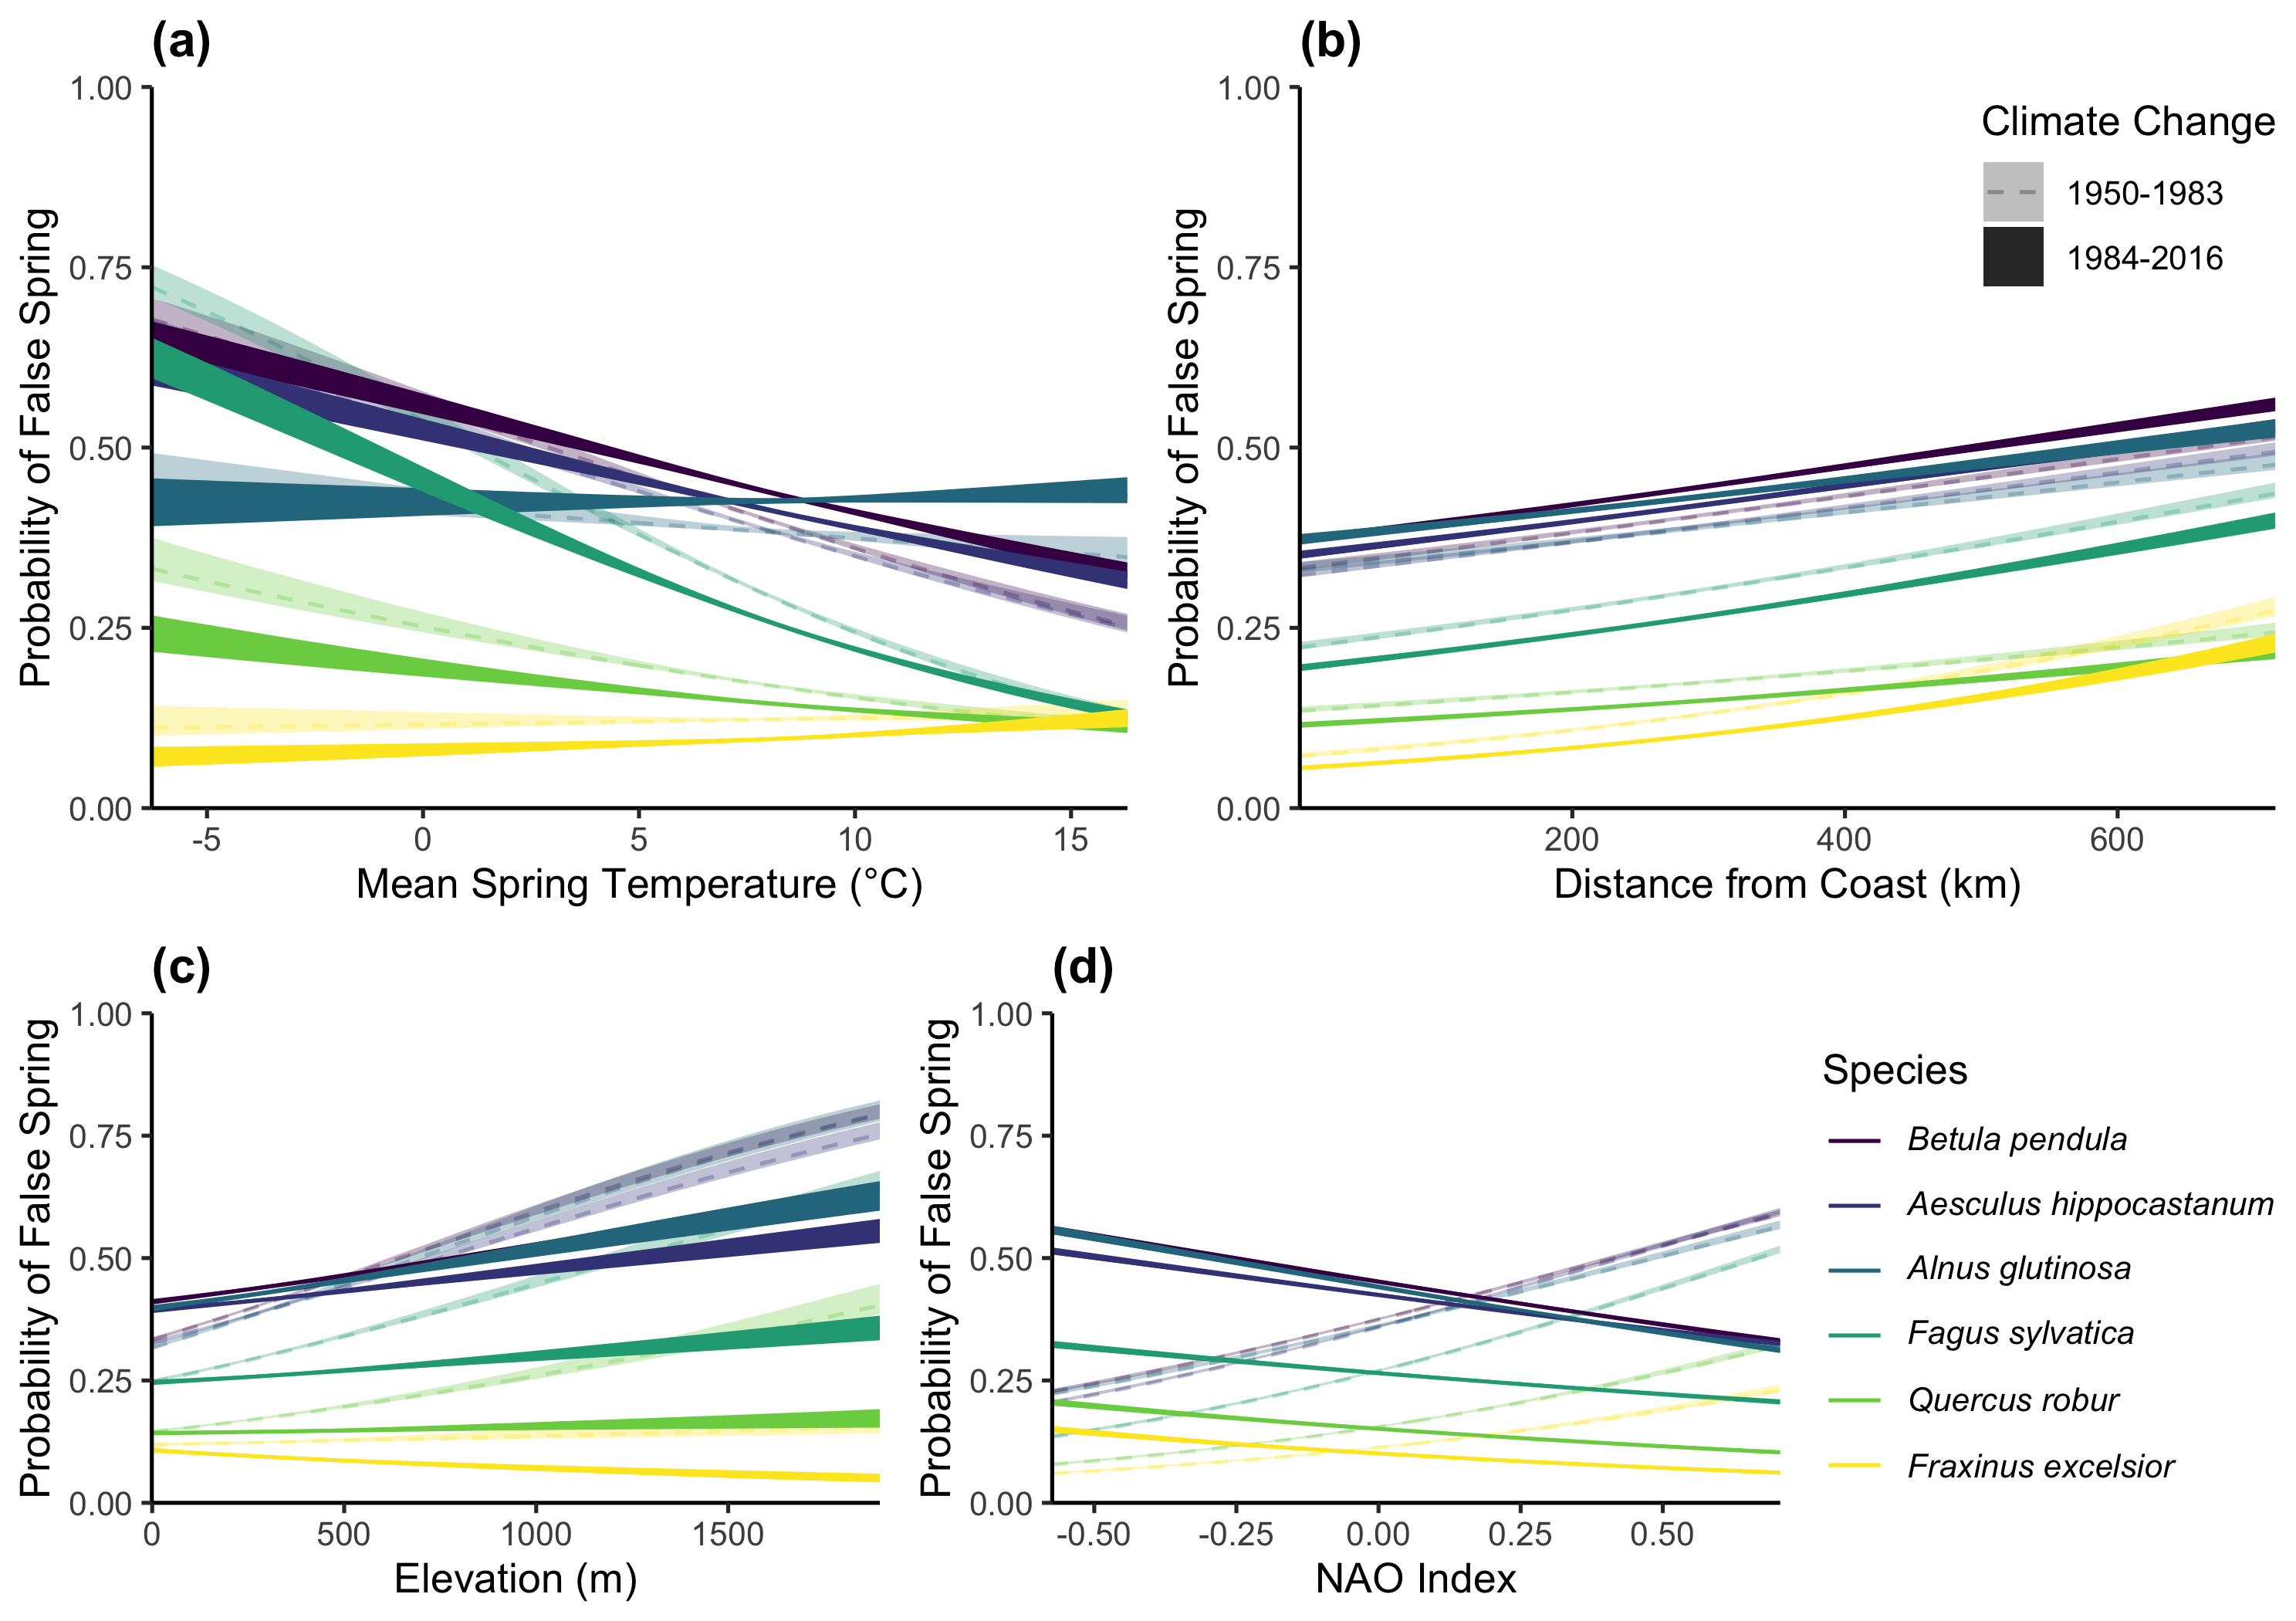
\includegraphics[width=16cm]{..//analyses/figures/APC_allpred_allspp_baseR_long98.png}
  -\caption{Average predictive comparisons for all climate change interactions with each of the main effects (i.e., mean spring temperature, distance from the coast, elevation, and NAO index) for all species. Shading around the lines represent the 98\% uncertainty intervals. }\label{fig:suppapc}
  -\end{center}
  -\end{figure}}
  
{\begin{figure} [H]
  -\begin{center}
  -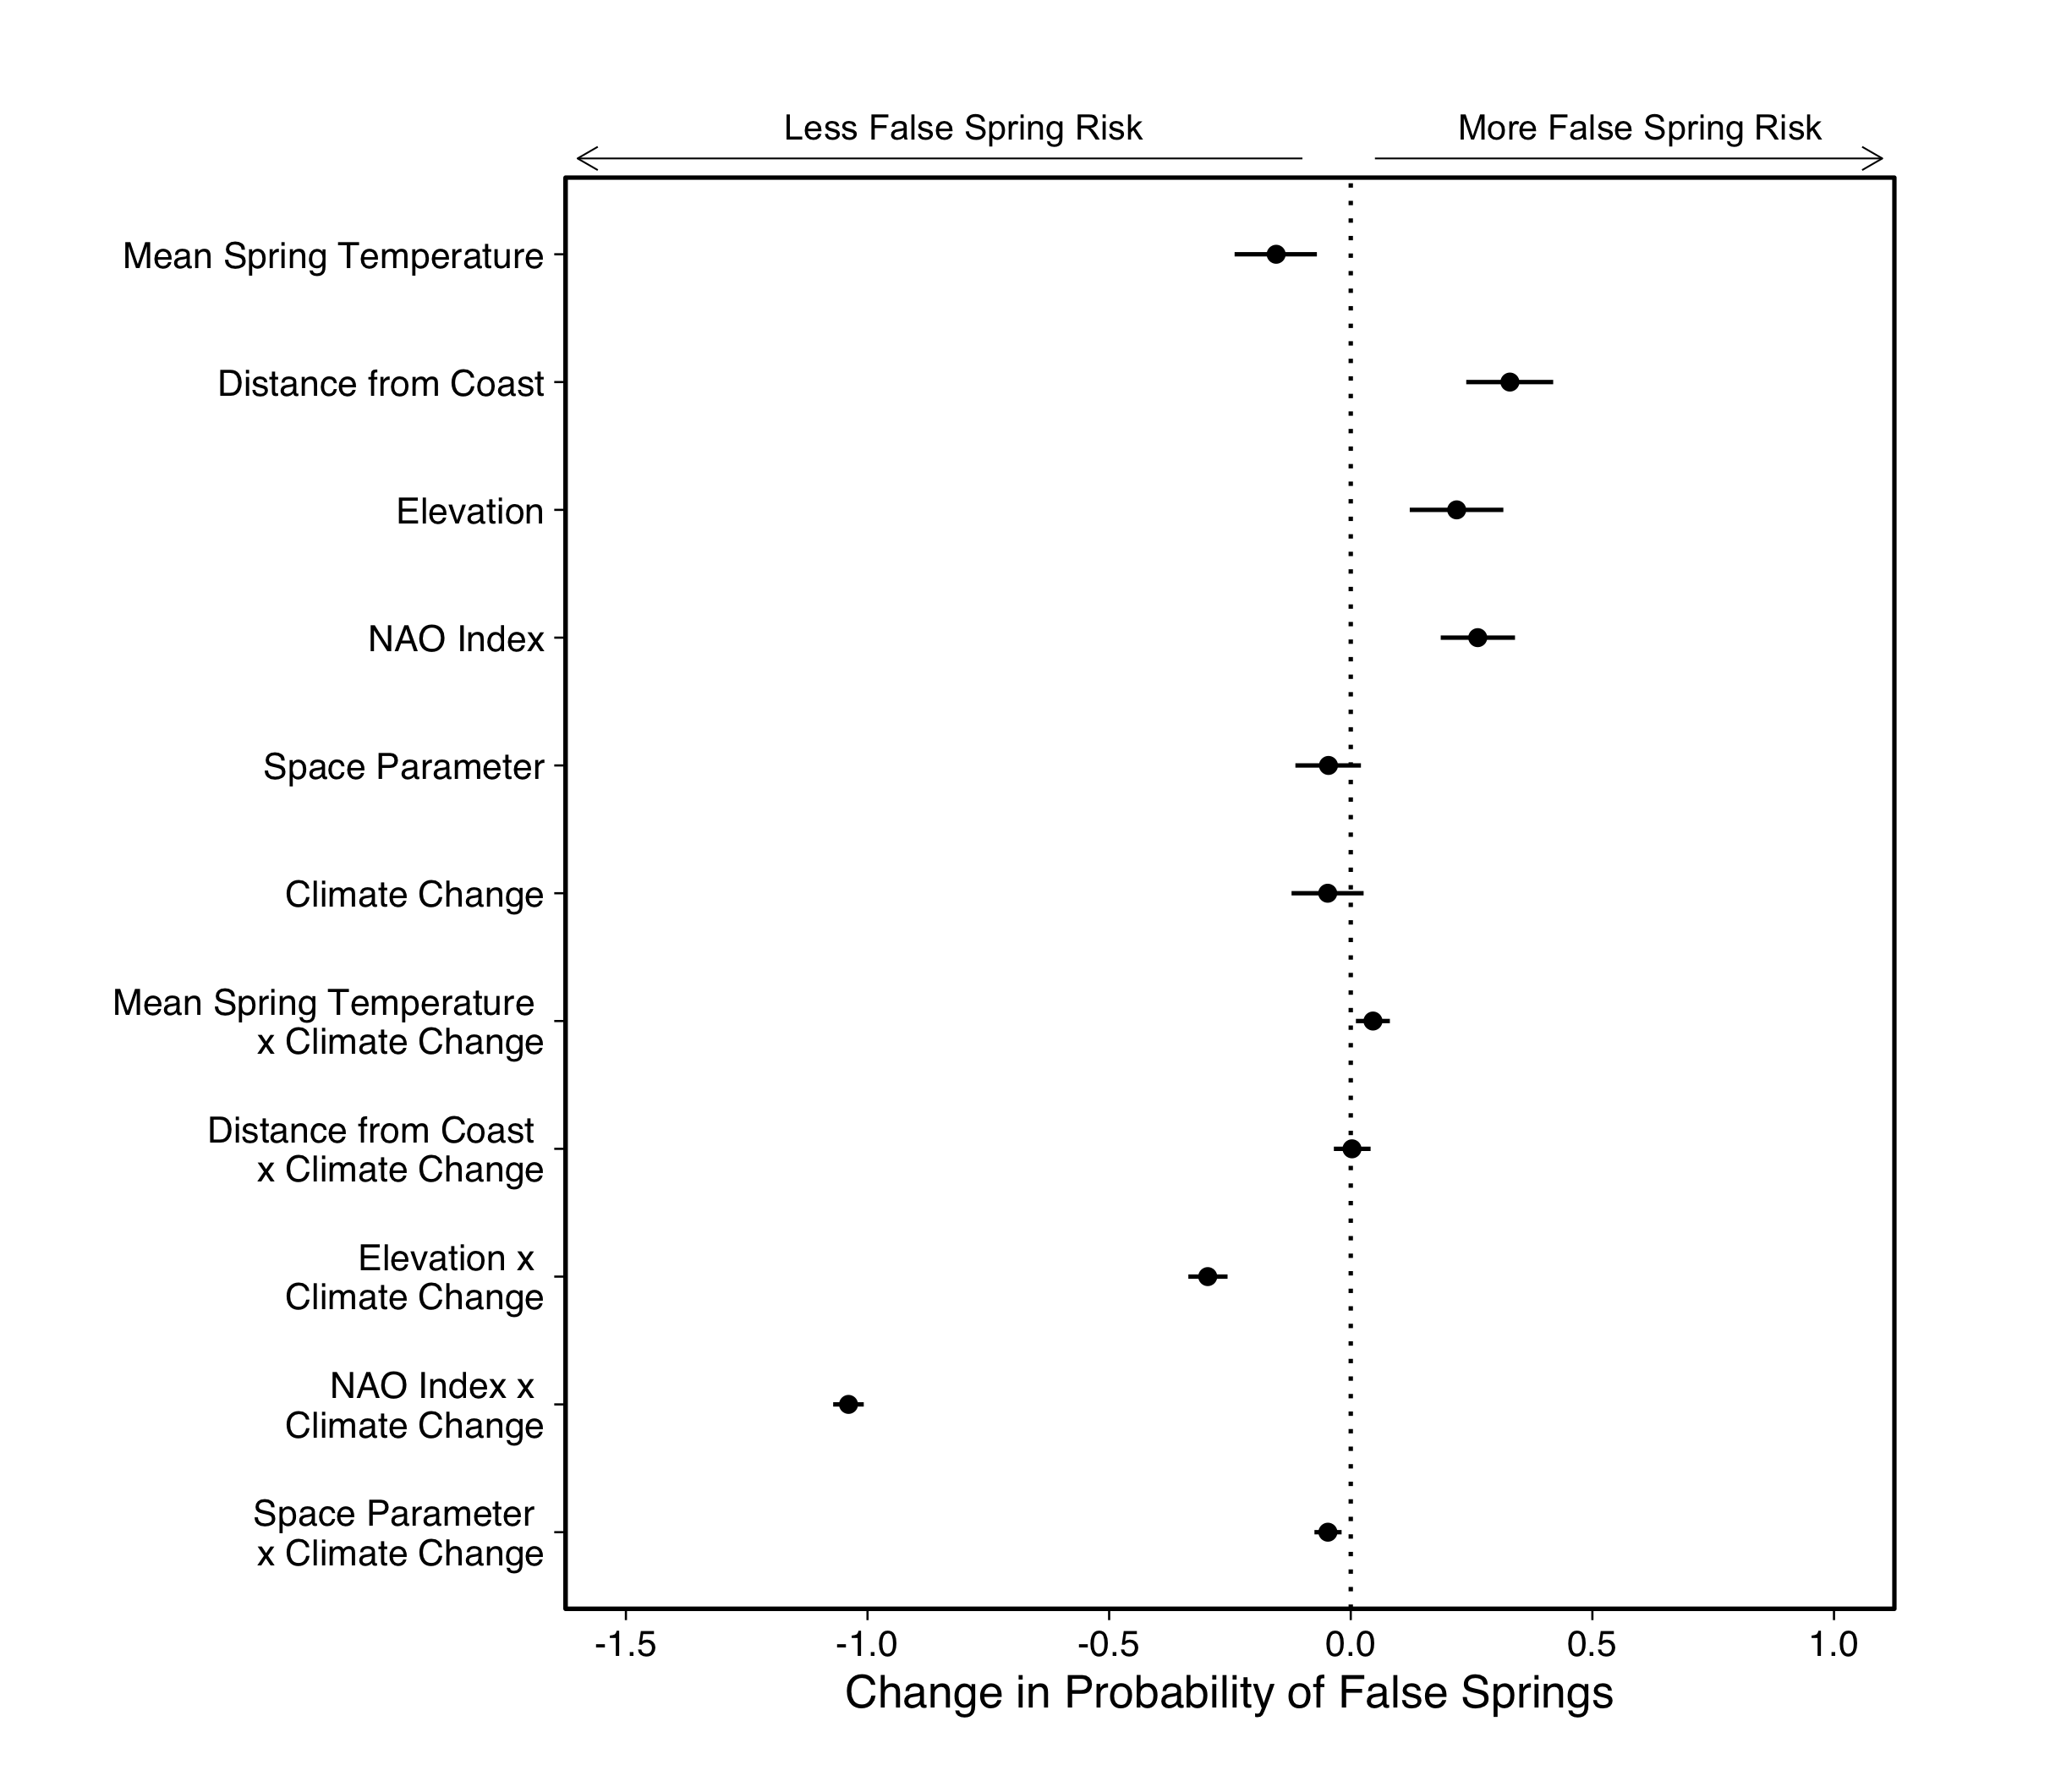
\includegraphics[width=12cm]{..//analyses/figures/model_output_98_dvrlong.png}
  -\caption{Effects of species, climatic and geographical predictors on false spring risk with different rates of leafout for each species. More positive values indicate an increased probability of a false spring whereas more negative values suggest a lower probability of a false spring. Dots and lines show means and 98\% uncertainty intervals. See Table \ref{tab:suppmoddvr} for full model output. }\label{fig:dvr}
  -\end{center}
  -\end{figure}}
  
\newpage
% latex table generated in R 3.6.0 by xtable 1.8-4 package
% Fri May 29 07:57:12 2020
\begin{longtable}{lrrrrrrr}
\caption{Summary of Bernoulli model of false spring risk with different rates of leafout for each species.} \\ 
  \hline
 & mean & 2\% & 10\% & 25\% & 75\% & 90\% & 98\% \\ 
  \hline \endhead  \hline
Intercept & -0.53 & -0.55 & -0.54 & -0.54 & -0.53 & -0.52 & -0.52 \\ 
  NAO Index & 0.27 & 0.25 & 0.25 & 0.27 & 0.28 & 0.30 & 0.30 \\ 
  Mean Spring 
Temperature & -0.24 & -0.27 & -0.26 & -0.25 & -0.23 & -0.21 & -0.21 \\ 
  Distance from 
Coast & 0.29 & 0.25 & 0.26 & 0.28 & 0.30 & 0.31 & 0.32 \\ 
  Elevation & 0.25 & 0.22 & 0.23 & 0.24 & 0.26 & 0.28 & 0.29 \\ 
  Space Parameter & -0.02 & -0.05 & -0.04 & -0.03 & -0.01 & -0.00 & 0.00 \\ 
  Climate Change & 0.13 & 0.10 & 0.11 & 0.12 & 0.13 & 0.15 & 0.15 \\ 
  \textit{Alnus glutinosa} & 0.13 & 0.11 & 0.12 & 0.12 & 0.14 & 0.15 & 0.15 \\ 
  \textit{Betula pendula} & 0.08 & 0.06 & 0.06 & 0.07 & 0.08 & 0.09 & 0.09 \\ 
  \textit{Fagus sylvatica} & -1.55 & -1.58 & -1.57 & -1.56 & -1.54 & -1.53 & -1.53 \\ 
  \textit{Fraxinus excelsior} & -2.32 & -2.36 & -2.35 & -2.33 & -2.31 & -2.29 & -2.28 \\ 
  \textit{Quercus robur} & -1.93 & -1.96 & -1.95 & -1.94 & -1.92 & -1.91 & -1.91 \\ 
  NAO Index
x\textit{ Alnus glutinosa} & -0.13 & -0.17 & -0.16 & -0.14 & -0.11 & -0.10 & -0.08 \\ 
  NAO Index
x\textit{ Betula pendula} & -0.07 & -0.11 & -0.10 & -0.08 & -0.06 & -0.04 & -0.03 \\ 
  NAO Index
x\textit{ Fagus sylvatica} & 0.19 & 0.13 & 0.15 & 0.17 & 0.20 & 0.23 & 0.25 \\ 
  NAO Index
x\textit{ Fraxinus excelsior} & -0.11 & -0.19 & -0.17 & -0.13 & -0.09 & -0.05 & -0.03 \\ 
  NAO Index
x\textit{ Quercus robur} & 0.05 & -0.01 & 0.01 & 0.03 & 0.07 & 0.10 & 0.11 \\ 
  Mean Spring 
Temperature
x\textit{ Alnus glutinosa} & 0.21 & 0.16 & 0.18 & 0.20 & 0.23 & 0.25 & 0.27 \\ 
  Mean Spring 
Temperature
x\textit{ Betula pendula} & -0.01 & -0.05 & -0.04 & -0.02 & 0.01 & 0.02 & 0.04 \\ 
  Mean Spring 
Temperature
x\textit{ Fagus sylvatica} & -0.17 & -0.23 & -0.21 & -0.19 & -0.15 & -0.13 & -0.11 \\ 
  Mean Spring 
Temperature
x\textit{ Fraxinus excelsior} & 0.40 & 0.30 & 0.33 & 0.37 & 0.43 & 0.47 & 0.49 \\ 
  Mean Spring 
Temperature
x\textit{ Quercus robur} & 0.06 & -0.01 & 0.01 & 0.04 & 0.08 & 0.11 & 0.13 \\ 
  Distance from 
Coast
x\textit{ Alnus glutinosa} & -0.05 & -0.10 & -0.09 & -0.06 & -0.03 & -0.01 & 0.01 \\ 
  Distance from 
Coast
x\textit{ Betula pendula} & 0.01 & -0.03 & -0.02 & -0.00 & 0.03 & 0.05 & 0.06 \\ 
  Distance from 
Coast
x\textit{ Fagus sylvatica} & 0.07 & 0.00 & 0.02 & 0.05 & 0.09 & 0.12 & 0.13 \\ 
  Distance from 
Coast
x\textit{ Fraxinus excelsior} & 0.29 & 0.19 & 0.22 & 0.26 & 0.32 & 0.36 & 0.39 \\ 
  Distance from 
Coast
x\textit{ Quercus robur} & -0.08 & -0.15 & -0.13 & -0.10 & -0.06 & -0.03 & -0.00 \\ 
  Elevation
x\textit{ Alnus glutinosa} & 0.10 & 0.03 & 0.05 & 0.08 & 0.12 & 0.14 & 0.16 \\ 
  Elevation
x\textit{ Betula pendula} & 0.05 & 0.00 & 0.01 & 0.04 & 0.06 & 0.09 & 0.10 \\ 
  Elevation
x\textit{ Fagus sylvatica} & -0.11 & -0.18 & -0.16 & -0.13 & -0.09 & -0.07 & -0.05 \\ 
  Elevation
x\textit{ Fraxinus excelsior} & -0.25 & -0.36 & -0.33 & -0.28 & -0.22 & -0.17 & -0.14 \\ 
  Elevation
x\textit{ Quercus robur} & 0.02 & -0.06 & -0.04 & -0.00 & 0.04 & 0.07 & 0.09 \\ 
  Space Parameter
x\textit{ Alnus glutinosa} & 0.00 & -0.04 & -0.03 & -0.01 & 0.01 & 0.03 & 0.04 \\ 
  Space Parameter
x\textit{ Betula pendula} & -0.01 & -0.04 & -0.03 & -0.02 & 0.00 & 0.02 & 0.03 \\ 
  Space Parameter
x\textit{ Fagus sylvatica} & -0.08 & -0.13 & -0.12 & -0.10 & -0.07 & -0.05 & -0.03 \\ 
  Space Parameter
x\textit{ Fraxinus excelsior} & -0.03 & -0.11 & -0.09 & -0.06 & -0.01 & 0.02 & 0.04 \\ 
  Space Parameter
x\textit{ Quercus robur} & -0.03 & -0.09 & -0.07 & -0.05 & -0.02 & 0.01 & 0.02 \\ 
  Climate Change
x\textit{ Alnus glutinosa} & 0.05 & 0.01 & 0.02 & 0.04 & 0.06 & 0.08 & 0.10 \\ 
  Climate Change
x\textit{ Betula pendula} & 0.05 & 0.01 & 0.02 & 0.04 & 0.06 & 0.07 & 0.09 \\ 
  Climate Change
x\textit{ Fagus sylvatica} & -0.34 & -0.39 & -0.38 & -0.36 & -0.32 & -0.30 & -0.29 \\ 
  Climate Change
x\textit{ Fraxinus excelsior} & -0.45 & -0.53 & -0.50 & -0.47 & -0.42 & -0.39 & -0.37 \\ 
  Climate Change
x\textit{ Quercus robur} & -0.35 & -0.41 & -0.39 & -0.37 & -0.33 & -0.31 & -0.29 \\ 
  NAO Index x Climate Change & -1.04 & -1.07 & -1.06 & -1.05 & -1.03 & -1.02 & -1.01 \\ 
  Mean Spring 
Temperature x Climate Change & 0.05 & 0.01 & 0.02 & 0.04 & 0.06 & 0.07 & 0.08 \\ 
  Distance from 
Coast x Climate Change & 0.00 & -0.03 & -0.02 & -0.01 & 0.01 & 0.03 & 0.04 \\ 
  Elevation x Climate Change & -0.30 & -0.34 & -0.32 & -0.31 & -0.28 & -0.27 & -0.25 \\ 
  Space Parameter x Climate Change & -0.05 & -0.08 & -0.07 & -0.06 & -0.04 & -0.03 & -0.02 \\ 
   \hline
\hline
\label{tab:suppmoddvr}
\end{longtable}

  
  {\begin{figure} [H]
  -\begin{center}
  -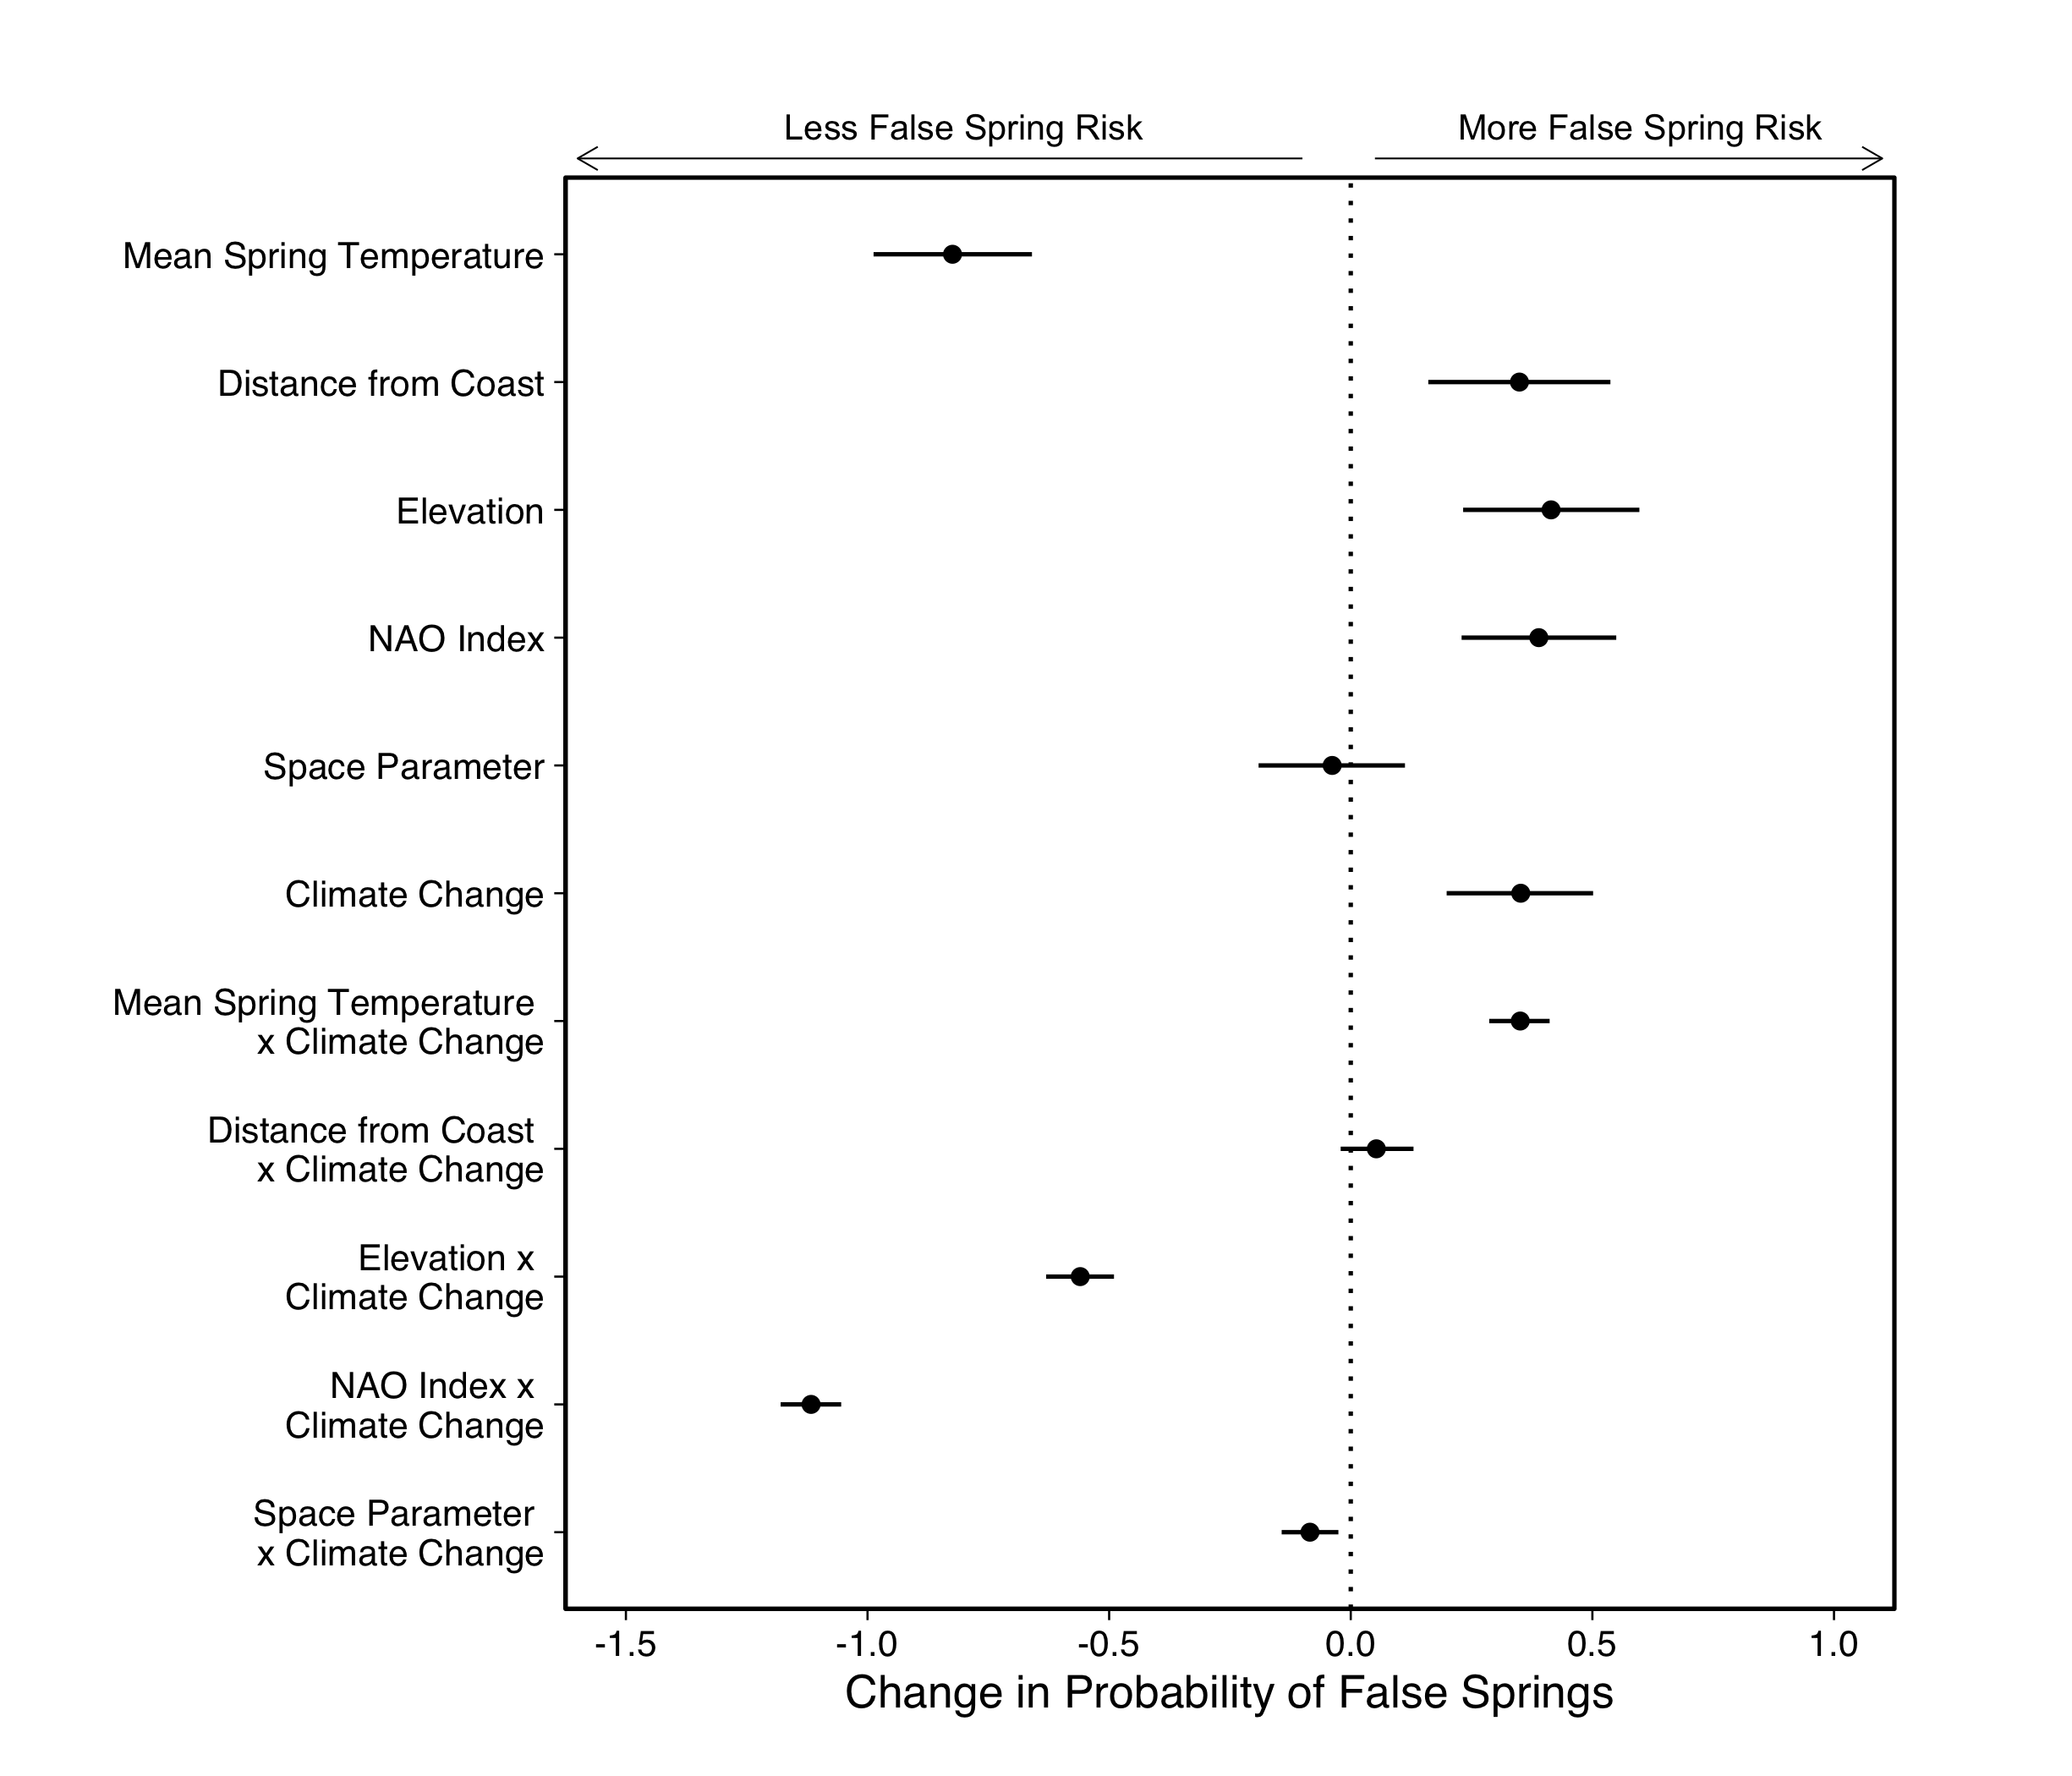
\includegraphics[width=12cm]{..//analyses/figures/model_output_98_fivelong.png}
  -\caption{Effects of species, climatic and geographical predictors on false spring risk with a lower temperature threshold (-5$^{\circ}$C) for defining a false spring. More positive values indicate an increased probability of a false spring whereas more negative values suggest a lower probability of a false spring. Dots and lines show means and 98\% uncertainty intervals. See Table \ref{tab:suppmodfive} for full model output. }\label{fig:five}
  -\end{center}
  -\end{figure}}
  
\newpage
\begin{kframe}


{\ttfamily\noindent\bfseries\color{errorcolor}{\#\# Error: '\textbackslash{}c' is an unrecognized escape in character string starting "{}"{}Summary of Bernoulli model of false spring risk with a lower temperature threshold (-5\$\textasciicircum{}\{\textbackslash{}c"{}}}\end{kframe}

  {\begin{figure} [H]
  -\begin{center}
  -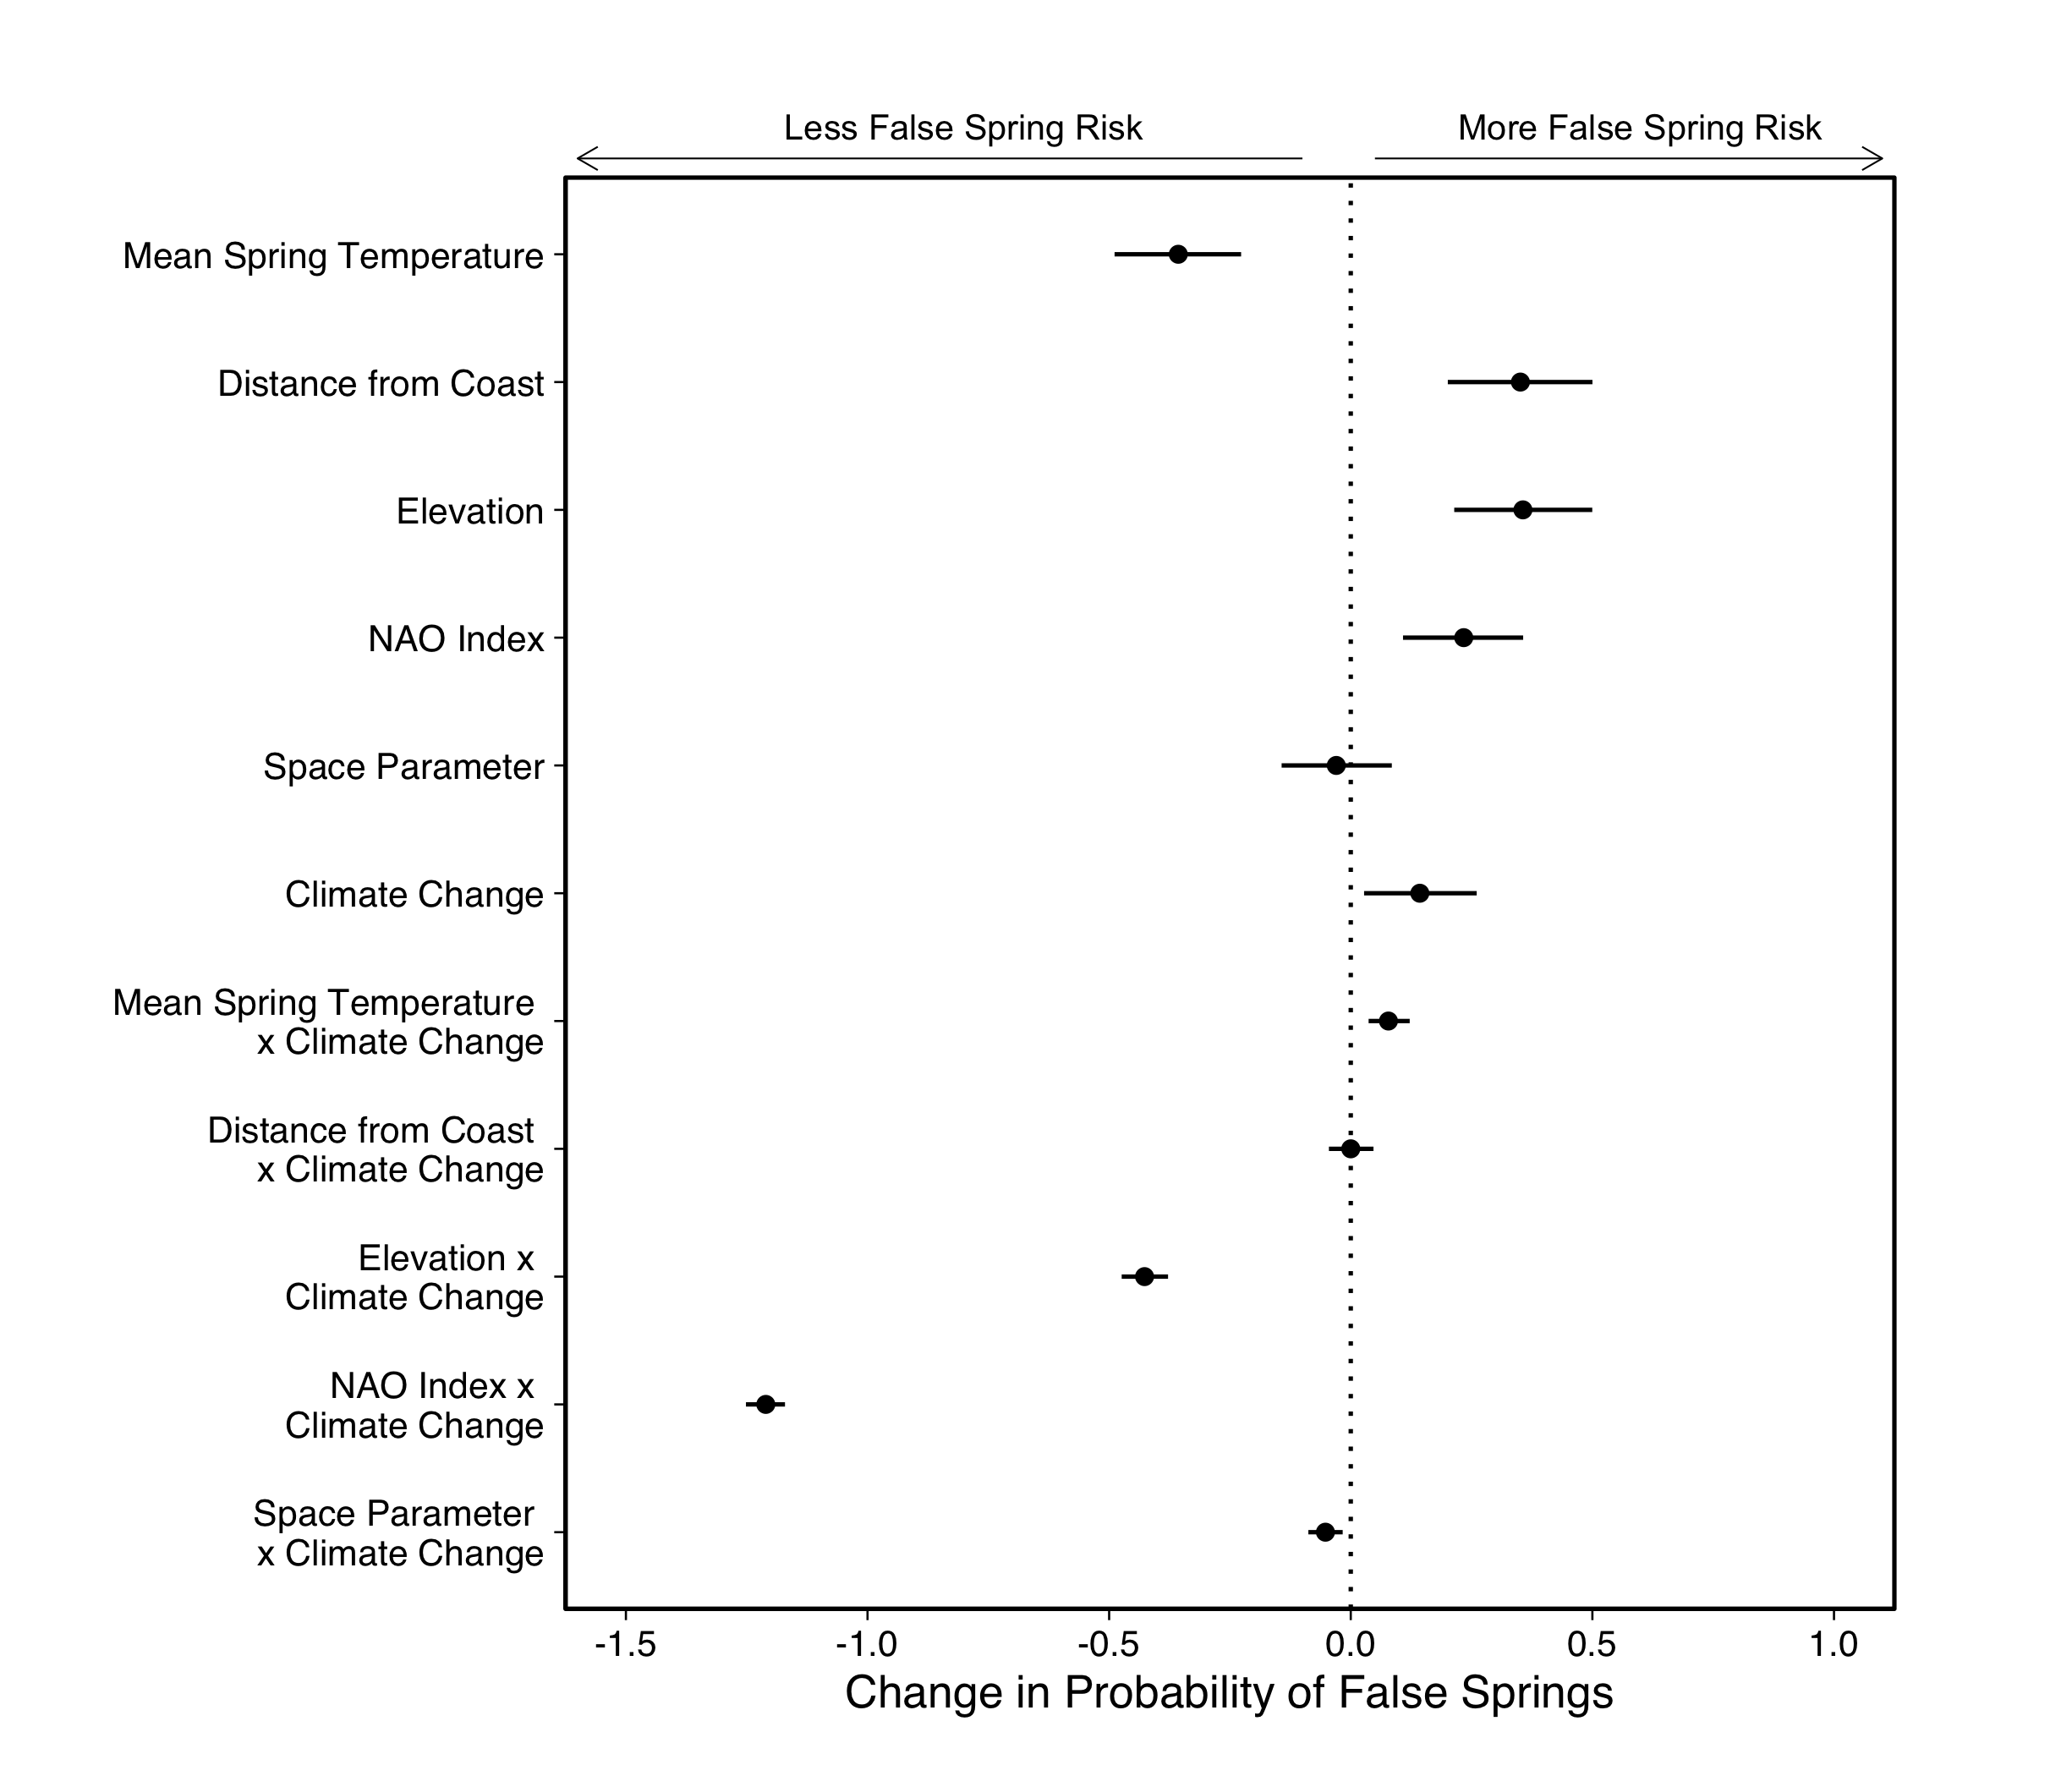
\includegraphics[width=12cm]{..//analyses/figures/model_output_98_longtemps.png}
  -\caption{Effects of species, climatic and geographical predictors on false spring risk with a lower temperature threshold (-5$^{\circ}$C) for early-leafout species (i.e., \textit{Aesculus hippocastanum}, \textit{Alnus glutinosa} and \textit{Betula pendula}) and a higher temperature threshold (-2.2$^{\circ}$C) for late-leafout species (i.e., \textit{Fagus sylvatica}, \textit{Fraxinus excelsior} and \textit{Quercus robur}). More positive values indicate an increased probability of a false spring whereas more negative values suggest a lower probability of a false spring. Dots and lines show means and 98\% uncertainty intervals. See Table \ref{tab:suppmodlongtemps} for full model output. }\label{fig:longtemps}
  -\end{center}
  -\end{figure}}
  
\newpage
\begin{kframe}


{\ttfamily\noindent\bfseries\color{errorcolor}{\#\# Error: '\textbackslash{}c' is an unrecognized escape in character string starting "{}"{}Summary of Bernoulli model of false spring risk with with a lower temperature threshold (-5\$\textasciicircum{}\{\textbackslash{}c"{}}}\end{kframe}
\end{document}
